% Numbers, tables and figures: assets/ch4/build_transfer_assets.py.
% Sources: research/lora-refit-transfer-2026-11-16/{results,error-results,similarity-results,
% koren-results,model-card}.json and the recorded scope decision. Hashes are in the generated files.
\subsubsection{Final Refit and Held-Source Transfer}\label{sec:transfer-refit}
The locked transfer above evaluates only the W5-D ridge, so it cannot say whether the adaptation
gain survives a change of population. Answering that required final models rather than fold models:
the matched comparison of Section~\ref{sec:lora-results} produces five outer-fold fits per seed,
none of which is a deployable model. A separate campaign therefore refitted both recipes on all
permitted W data and scored the held source once.

\paragraph{Protocol.}
The locked protocol and the refit design are described with the methods in
Section~\ref{sec:refit-protocol}. The transfer set had been inspected in earlier work, so this is a
post-hoc transfer evaluation on a previously examined held-out source and not independent external
validation. This boundary is limitation L1 in Table~\ref{tab:transfer-limits} and is repeated with
every claim below.

\paragraph{Transfer result.}
The primary endpoint is the peptide-macro mean absolute error on the replicate-1 transfer cohort of
\nTCells{} cells, \nTPeptides{} peptides and \nTGroups{} protein groups. Table~\ref{tab:transfer-main}
and Figure~\ref{fig:transfer-contrasts} report it together with the two baselines that were fixed in
advance and the constant predictor. LoRA-D reaches MAE \nTLoraMae{}, against \nTFrozenMae{} for its
matched frozen control, \nTWfiveMae{} for the locked W5-D ridge and \nTZeroMae{} for predicting no
effect at all. Rank behaviour moves in the same direction: Spearman \nTLoraRho{} and positive-event
AUROC \nTLoraAuc{}.

\begin{figure}[htbp]
  \centering
  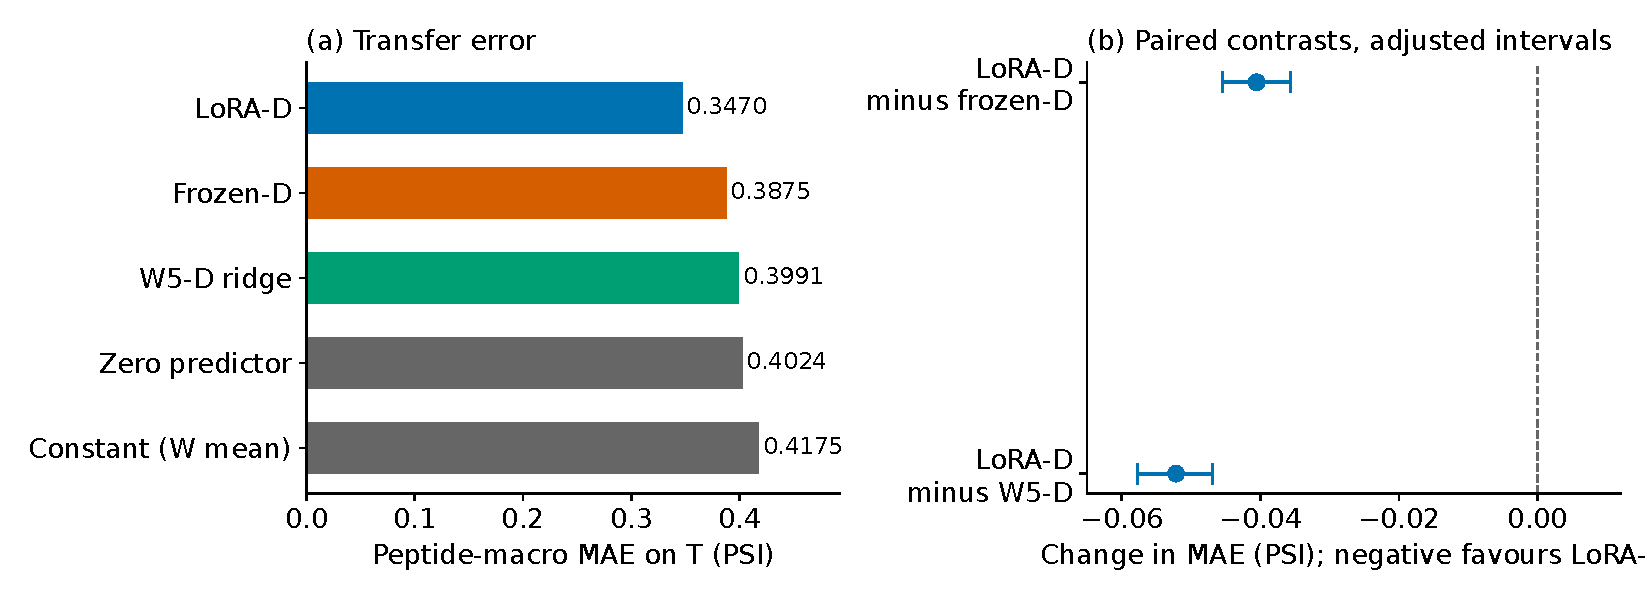
\includegraphics[width=\textwidth]{assets/ch4/fig-transfer-contrasts.pdf}
  \caption[Transfer error and prespecified contrasts]{Transfer error and prespecified contrasts. (a) Peptide-macro MAE on the held source for
  the adapted model, its matched control and the fixed baselines; (b) the two paired differences
  with multiplicity-adjusted protein-group bootstrap intervals. Panel (b) shows the same two
  comparisons as Table~\ref{tab:transfer-contrasts}, not a per-peptide spread.}
  \label{fig:transfer-contrasts}
\end{figure}

\begin{table}[htbp]
  \centering
  \caption[Held-source transfer results after the final refit]{Held-source transfer results after the final refit. MAE and RMSE are lower-is-better in
  PSI units; Spearman and positive-event AUROC are higher-is-better. Brier is the three-class score.
  Rank statistics are undefined for the two constant predictors.}
  \label{tab:transfer-main}
  % Generated by build_transfer_assets.py
% results: research/lora-refit-transfer-2026-11-16/results.json sha256 9a5b0036eb2b43b7574c7c567cead1dc2e253fe5405a081a658878878c104d5c
% errors: research/lora-refit-transfer-2026-11-16/error-results.json sha256 475be8f38f48629aadca00741e89c2ca8a099487c1f33c767bac149eeb9d2b8f
% similarity: research/lora-refit-transfer-2026-11-16/similarity-results.json sha256 0c1bfca1abb5a67a880aade48fca996bfe0a529d883e499a81dbd5e2e3a471f9
% koren: research/lora-refit-transfer-2026-11-16/koren-results.json sha256 2938dcf5225bd55b6060169dde3a0b5978d72e2c7658e6b7fe728f391b715368
% card: research/lora-refit-transfer-2026-11-16/model-card.json sha256 ea925afa4b961d8a09f06e145151bd8c4b8477fb5db40e6810f21979312ccd3d
% decision: research/g2-acceptance-2026-11-07/d4-decision-2026-11-17.md sha256 d79fd8cd4be420460cffb5c239c3a275309151cc62be6588aec301138bc88acc
% latency: system/app/tests/results/latency-lora.json sha256 9fedb6797d7e08184e162c5ee0ef0f3dea3e179407986654d8ee7b3799681479

{\small\setlength{\tabcolsep}{4pt}
\begin{tabularx}{\textwidth}{Xrrrrr}
\toprule
Model & MAE & RMSE & Spearman & AUROC$+$ & Brier \\
\midrule
LoRA-D & 0.3470 & 0.4297 & 0.4637 & 0.9083 & 0.1100 \\
Frozen-D & 0.3875 & 0.4798 & 0.4134 & 0.8745 & 0.1271 \\
W5-D ridge & 0.3991 & 0.4942 & 0.3781 & 0.8405 & 0.1291 \\
Zero predictor & 0.4024 & 0.5142 & -- & 0.5000 & -- \\
Constant (W mean) & 0.4175 & 0.5215 & -- & 0.5000 & -- \\
\bottomrule
\end{tabularx}}

\end{table}

Both prespecified contrasts favour the adapted model throughout their intervals
(Table~\ref{tab:transfer-contrasts}). The paired difference against the frozen control is
\nTDeltaFrozen{} with adjusted interval \nTDeltaFrozenCI{}, and against the locked ridge
\nTDeltaWfive{} with \nTDeltaWfiveCI{}. Intervals come from \nTBootstrap{} paired bootstrap
resamples of protein groups \citep{efron1979}, with the two-sided level corrected for the family of
two tests. The resampling is conditional on the fitted predictions, so it excludes the uncertainty
of training and model selection, and the three seeds share one outer partition rather than forming
three independent cohorts (L2).

\begin{table}[htbp]
  \centering
  \caption[Prespecified transfer contrasts]{Prespecified transfer contrasts. Negative differences favour LoRA-D. The adjusted
  interval corrects the two-sided level for the family of two comparisons; a confidence interval
  that excludes zero is not a statement about effect size in a new assay.}
  \label{tab:transfer-contrasts}
  % Generated by build_transfer_assets.py
% results: research/lora-refit-transfer-2026-11-16/results.json sha256 9a5b0036eb2b43b7574c7c567cead1dc2e253fe5405a081a658878878c104d5c
% errors: research/lora-refit-transfer-2026-11-16/error-results.json sha256 475be8f38f48629aadca00741e89c2ca8a099487c1f33c767bac149eeb9d2b8f
% similarity: research/lora-refit-transfer-2026-11-16/similarity-results.json sha256 0c1bfca1abb5a67a880aade48fca996bfe0a529d883e499a81dbd5e2e3a471f9
% koren: research/lora-refit-transfer-2026-11-16/koren-results.json sha256 2938dcf5225bd55b6060169dde3a0b5978d72e2c7658e6b7fe728f391b715368
% card: research/lora-refit-transfer-2026-11-16/model-card.json sha256 ea925afa4b961d8a09f06e145151bd8c4b8477fb5db40e6810f21979312ccd3d
% decision: research/g2-acceptance-2026-11-07/d4-decision-2026-11-17.md sha256 d79fd8cd4be420460cffb5c239c3a275309151cc62be6588aec301138bc88acc
% latency: system/app/tests/results/latency-lora.json sha256 9fedb6797d7e08184e162c5ee0ef0f3dea3e179407986654d8ee7b3799681479

{\small\setlength{\tabcolsep}{4pt}
\begin{tabularx}{\textwidth}{Xrll}
\toprule
Contrast & $\Delta$MAE & 95\% interval & Adjusted interval \\
\midrule
LoRA-D minus frozen-D & -0.0405 & [-0.0449, -0.0362] & [-0.0455, -0.0356] \\
LoRA-D minus W5-D & -0.0522 & [-0.0569, -0.0475] & [-0.0577, -0.0469] \\
\bottomrule
\end{tabularx}}

\end{table}

\paragraph{Where the advantage disappears.}
The average hides a reversal. Table~\ref{tab:transfer-strata} and Figure~\ref{fig:transfer-strata}
split the cohort by the measured wild-type stability of the scanning peptide. The advantage of
LoRA-D over predicting nothing falls monotonically as that stability rises and then changes sign:
in the highest stratum, \nTGtFiveN{} peptides in \nTGtFiveGroups{} groups, the zero predictor
reaches MAE \nTGtFiveZero{} against \nTGtFiveLora{} for LoRA-D, a difference of \nTGtFiveDelta{}
with adjusted interval \nTGtFiveCI{} lying entirely above zero. This unfavourable result is
therefore not sampling noise, and it is recorded as limitation L3 rather than being left out of the
comparison. The two weaker models fail in the same region by a wider margin, which makes the
stratum a property of the task rather than of the adapter alone.

\begin{figure}[htbp]
  \centering
  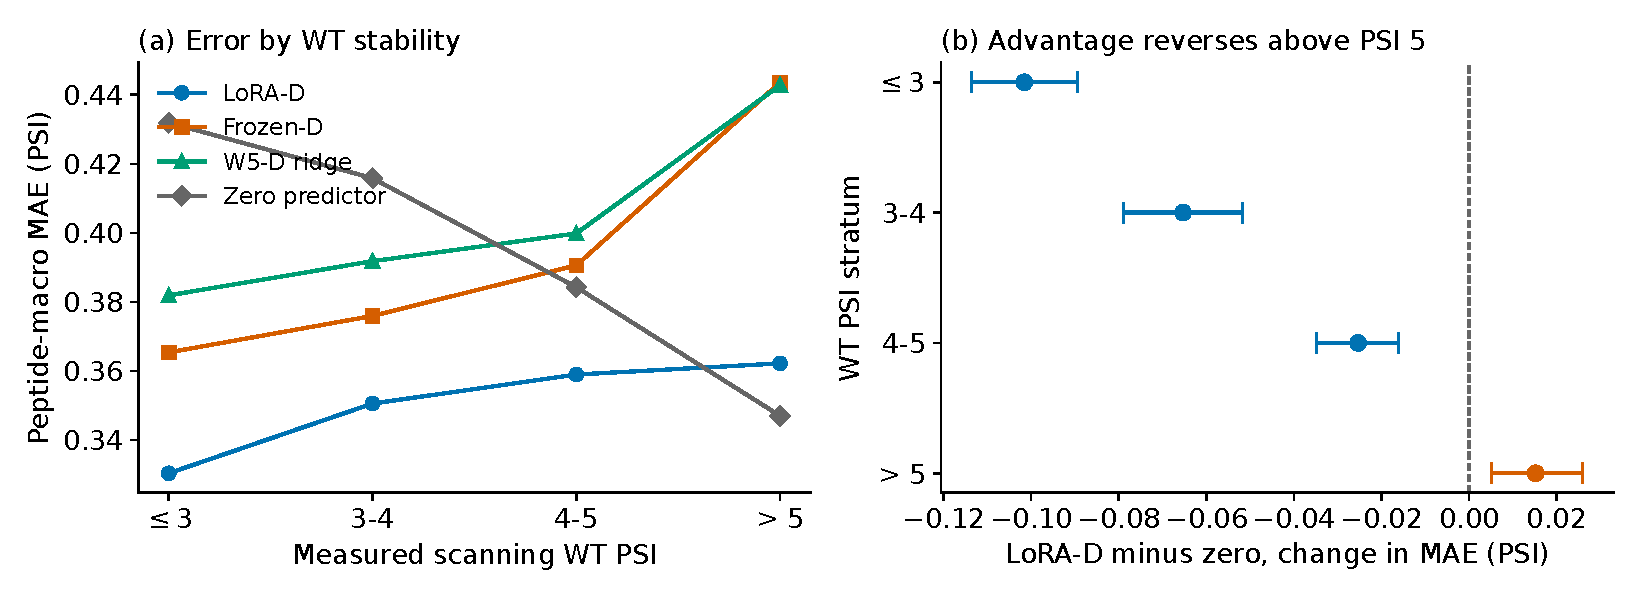
\includegraphics[width=\textwidth]{assets/ch4/fig-transfer-strata.pdf}
  \caption[The transfer advantage reverses in stable peptides]{The transfer advantage reverses in stable peptides. (a) Peptide-macro MAE of each model by
  measured wild-type PSI; (b) the paired difference against the zero predictor with adjusted
  intervals, where the highest stratum lies entirely above zero. Panel (a) joins points of one
  model and the connectors are not intervals.}
  \label{fig:transfer-strata}
\end{figure}

\paragraph{Diagnosis of the reversal.}
Four candidate explanations were examined, each with its own test. The signed-residual table shows a
directional mismatch in the highest stratum: the measured mean effect there is \nTGtFiveTarget{}
while the mean prediction is \nTGtFivePred{}, so the models keep predicting stabilisation in a
region where the measured effects are destabilising on average. The published score shift between
out-of-fold W, in-sample final W and the transfer cohort is reported without fitting any correction
on T. Replicate disagreement is reported as an indicator and is not treated as a known measurement
variance. The fourth candidate, construct similarity, needed a separate test and is treated next.
These are associations; the recorded status of the diagnosis is descriptive rather than causal, and
the mechanism remains unresolved. Reporting an unresolved mechanism is preferable to selecting the
one explanation that happens to fit.

\begin{table}[htbp]
  \centering
  \caption[Transfer error by measured wild-type stability]{Transfer error by measured wild-type stability. $n$ counts peptides. The last two columns
  are the paired LoRA-D-minus-zero difference and its adjusted protein-group interval; a positive
  difference means the zero predictor is better. Stratum intervals are exploratory.}
  \label{tab:transfer-strata}
  % Generated by build_transfer_assets.py
% results: research/lora-refit-transfer-2026-11-16/results.json sha256 9a5b0036eb2b43b7574c7c567cead1dc2e253fe5405a081a658878878c104d5c
% errors: research/lora-refit-transfer-2026-11-16/error-results.json sha256 475be8f38f48629aadca00741e89c2ca8a099487c1f33c767bac149eeb9d2b8f
% similarity: research/lora-refit-transfer-2026-11-16/similarity-results.json sha256 0c1bfca1abb5a67a880aade48fca996bfe0a529d883e499a81dbd5e2e3a471f9
% koren: research/lora-refit-transfer-2026-11-16/koren-results.json sha256 2938dcf5225bd55b6060169dde3a0b5978d72e2c7658e6b7fe728f391b715368
% card: research/lora-refit-transfer-2026-11-16/model-card.json sha256 ea925afa4b961d8a09f06e145151bd8c4b8477fb5db40e6810f21979312ccd3d
% decision: research/g2-acceptance-2026-11-07/d4-decision-2026-11-17.md sha256 d79fd8cd4be420460cffb5c239c3a275309151cc62be6588aec301138bc88acc
% latency: system/app/tests/results/latency-lora.json sha256 9fedb6797d7e08184e162c5ee0ef0f3dea3e179407986654d8ee7b3799681479

{\small\setlength{\tabcolsep}{4pt}
\begin{tabularx}{\textwidth}{lrrrrrrl}
\toprule
WT PSI & $n$ & Zero & W5-D & Frozen-D & LoRA-D & $\Delta$ & Adjusted interval \\
\midrule
$\le 3$ & 524 & 0.4319 & 0.3819 & 0.3654 & 0.3303 & -0.1016 & [-0.1136, -0.0895] \\
$3<\mathrm{PSI}\le4$ & 323 & 0.4158 & 0.3918 & 0.3759 & 0.3505 & -0.0653 & [-0.0789, -0.0517] \\
$4<\mathrm{PSI}\le5$ & 306 & 0.3843 & 0.3998 & 0.3906 & 0.3589 & -0.0253 & [-0.0348, -0.0161] \\
$>5$ & 257 & 0.3470 & 0.4428 & 0.4436 & 0.3622 & 0.0152 & [0.0051, 0.0260] \\
\bottomrule
\end{tabularx}}

\end{table}


\paragraph{Is the gain just sequence similarity?}
A plausible objection is that the adapted model does well on the transfer cohort only because some
of its peptides resemble training peptides. This was tested with a criterion fixed before the
numbers were computed, using the maximum aligned identity of each transfer peptide against the
\nVthreeNPeptides{} training peptides. Table~\ref{tab:transfer-similarity} reports the contrasts
within identity bins. In the least similar bin, \nTBottomBinN{} peptides in \nTBottomBinGroups{}
groups, the difference against the frozen control is still \nTBottomBinDelta{} with adjusted
interval \nTBottomBinCI{} below zero, and the rank correlation between identity and advantage is
\nTSimRho{} ($p=\nTSimRhoP{}$), which is near zero and of the opposite sign to the objection.
The recorded verdict is therefore that local similarity to the training peptides does not explain
the observed advantage. Two qualifications matter: the observed identity range of the cohort is only
\nTIdentityMin{} to \nTIdentityMax{}, so the two highest bins are empty and the test covers a narrow
range; and a proxy for local identity cannot exclude remote homology or exposure of these sequences
in the pretraining corpus of the backbone \citep{bernett2024}.

\begin{table}[htbp]
  \centering
  \caption[Transfer contrasts within sequence-identity bins]{Transfer contrasts within sequence-identity bins. Identity is the maximum aligned identity
  of a transfer peptide against the training peptides. Bins were fixed before computation and the
  two highest bins contain no data. Intervals adjust for four comparisons.}
  \label{tab:transfer-similarity}
  % Generated by build_transfer_assets.py
% results: research/lora-refit-transfer-2026-11-16/results.json sha256 9a5b0036eb2b43b7574c7c567cead1dc2e253fe5405a081a658878878c104d5c
% errors: research/lora-refit-transfer-2026-11-16/error-results.json sha256 475be8f38f48629aadca00741e89c2ca8a099487c1f33c767bac149eeb9d2b8f
% similarity: research/lora-refit-transfer-2026-11-16/similarity-results.json sha256 0c1bfca1abb5a67a880aade48fca996bfe0a529d883e499a81dbd5e2e3a471f9
% koren: research/lora-refit-transfer-2026-11-16/koren-results.json sha256 2938dcf5225bd55b6060169dde3a0b5978d72e2c7658e6b7fe728f391b715368
% card: research/lora-refit-transfer-2026-11-16/model-card.json sha256 ea925afa4b961d8a09f06e145151bd8c4b8477fb5db40e6810f21979312ccd3d
% decision: research/g2-acceptance-2026-11-07/d4-decision-2026-11-17.md sha256 d79fd8cd4be420460cffb5c239c3a275309151cc62be6588aec301138bc88acc
% latency: system/app/tests/results/latency-lora.json sha256 9fedb6797d7e08184e162c5ee0ef0f3dea3e179407986654d8ee7b3799681479

{\small\setlength{\tabcolsep}{4pt}
\begin{tabularx}{\textwidth}{Xlrrrl}
\toprule
Contrast & Identity bin & Peptides & Groups & $\Delta$MAE & Adjusted interval \\
\midrule
LoRA-D minus frozen-D & [0.0, 0.25) & 1093 & 627 & -0.0399 & [-0.0457, -0.0342] \\
LoRA-D minus frozen-D & [0.25, 0.5) & 317 & 239 & -0.0427 & [-0.0564, -0.0293] \\
LoRA-D minus W5-D & [0.0, 0.25) & 1093 & 627 & -0.0542 & [-0.0609, -0.0472] \\
LoRA-D minus W5-D & [0.25, 0.5) & 317 & 239 & -0.0452 & [-0.0588, -0.0318] \\
\bottomrule
\end{tabularx}}

\end{table}

\paragraph{A survey outside the construct.}
An additional C-terminal degron data set \citep{koren2018} was scored rank-only within each
substrate, covering \nTKorenSubstrates{} substrates and \nTKorenMutants{} mutants. Macro rank
agreement is weak, \nTKorenLora{} for LoRA-D and \nTKorenFrozen{} for the frozen control, and
negative for some substrates (Appendix~\ref{app:supplementary}). The interpretation rule for this
source was written down before any model was scored: because the data use a different degron class,
a different construct length and a three-bin scale, a weak result there does not refute the model
and only a strong positive result would have extended the claim. That asymmetry is kept here, so
the survey neither supports generalisation nor withdraws the development result (L4, L8). The source
had also failed an earlier admission gate for use as a validation cohort, because it contributes too
few new protein clusters.

\paragraph{Probabilities.}
Calibration again improves and degrades at the same time. The three-class Brier score falls from
\nTWfiveBrier{} for the locked ridge to \nTLoraBrier{} for the adapted model, while the
positive-event calibration error rises from \nTWfiveEce{} to \nTLoraEce{} (L5). The negative
direction stays weak, with AUROC \nTLoraAucMinus{} on the \nTMinusEligible{} peptides that are
eligible for it (L6). A single summary score is therefore not sufficient evidence that the
probabilities are usable.

\paragraph{What this permits to be claimed, and what it does not.}
With these results the author recorded a scope decision: the methodological and evaluation
contribution is accepted within the development setting, namely that adapting a protein language
model with a low-rank adapter lowers the error of single-substitution effect prediction for degron
reporter peptides, with matched controls and protein-group intervals, on the development
out-of-fold data and on the post-hoc held-source cohort. The decision was taken with the
limitations of Table~\ref{tab:transfer-limits} already known, and the supervisor's acknowledgement
of that record is still outstanding at this cutoff. It explicitly does not close the deployment
gate, does not change the served model, does not close the outstanding external-source and
structure extensions, and does not alter the recorded status of the campaign, which remains a
development result rather than a gate closure. Claims such as confirmation on an independent
source, generalisation to degrons in general, or readiness for deployment are not supported by
anything in this section.

% Generated by build_transfer_assets.py
% results: research/lora-refit-transfer-2026-11-16/results.json sha256 9a5b0036eb2b43b7574c7c567cead1dc2e253fe5405a081a658878878c104d5c
% errors: research/lora-refit-transfer-2026-11-16/error-results.json sha256 475be8f38f48629aadca00741e89c2ca8a099487c1f33c767bac149eeb9d2b8f
% similarity: research/lora-refit-transfer-2026-11-16/similarity-results.json sha256 0c1bfca1abb5a67a880aade48fca996bfe0a529d883e499a81dbd5e2e3a471f9
% koren: research/lora-refit-transfer-2026-11-16/koren-results.json sha256 2938dcf5225bd55b6060169dde3a0b5978d72e2c7658e6b7fe728f391b715368
% card: research/lora-refit-transfer-2026-11-16/model-card.json sha256 ea925afa4b961d8a09f06e145151bd8c4b8477fb5db40e6810f21979312ccd3d
% decision: research/g2-acceptance-2026-11-07/d4-decision-2026-11-17.md sha256 d79fd8cd4be420460cffb5c239c3a275309151cc62be6588aec301138bc88acc
% latency: system/app/tests/results/latency-lora.json sha256 9fedb6797d7e08184e162c5ee0ef0f3dea3e179407986654d8ee7b3799681479

{\small
\begin{longtable}{P{0.8cm}P{12.2cm}}
\caption{Limitations recorded with the scope decision}\label{tab:transfer-limits}\\
\toprule ID & Limitation \\
\midrule\endfirsthead
\caption[]{Limitations recorded with the scope decision (continued)}\\
\toprule ID & Limitation \\
\midrule\endhead
L1 & T was examined in earlier work, so this is a post-hoc transfer evaluation on a held-out source, not independent external validation. \\
L2 & The bootstrap conditions on the fitted predictions and excludes training and model-selection uncertainty. The three seeds share one outer partition. \\
L3 & In the WT-PSI $>5$ stratum the zero predictor has lower MAE than LoRA-D; frozen-D and W5-D are worse still. \\
L4 & The Koren survey gives weak rank agreement, negative for some substrates, on a different degron class, length and three-bin scale. \\
L5 & Positive-event calibration error of LoRA-D is worse than W5-D although its Brier score is better. \\
L6 & The negative direction stays weak and only 85 peptides are eligible for it. \\
L7 & Final predictions on W are in sample; the score shift is published and is not corrected using T. \\
L8 & One Koren substrate protein also occurs in the Zhang data, so the nine substrates are not fully independent. \\
L9 & The earlier verdict on the training-coverage family is unchanged; the LoRA result does not replace it. \\
L10 & Cross-runtime parity was outstanding when the decision was recorded, and no wet-lab or resource benefit of this project has been demonstrated. \\
\bottomrule
\end{longtable}}


\paragraph{Why the better model is still not the served model.}
The research pipeline now delivers what the earlier review found missing: identified checkpoints, a
calibrator with a recorded fit population, and inference parity. Parity was checked twice, first
between two execution paths of the research implementation on the same runtime over \nTParityRows{}
cells, and then between the recorded campaign runtime and the application host, where the maximum
absolute difference is $3.0\times10^{-6}$ against a tolerance of $10^{-5}$. A third check compares
the independent serving implementation with the research fixture over two complete tiles and finds
no difference at all.

Serving cost, however, decides against promotion for now. On the recorded local host the ridge
service answers a tile in \nTLatRidge{}~ms at the 95th percentile, whereas the adapted model needs
\nTLatLora{}~s, about \nTLatRatio{} times longer, because each tile requires three seeds of forward
passes over all 532 substitutions on a processor without acceleration. That misses the proposed
local target of \nTLatTarget{}~ms by two orders of magnitude and would make whole-protein jobs
impractical. The adapted model is therefore registered as a selectable candidate while the
calibrated ridge remains the default of the delivered configuration, which keeps the research result
and the deployment decision separate (L10). The author has since set the adapted model as default
on one local installation by configuration; no serving decision record or supervisor approval exists
for that setting, and it does not change the status of any result in this section.
